%%%%%%%%%%%%%%%%%%%%%%%%%%%%%%%%%%%%%%%%%
% Beamer Presentation
% LaTeX Template
% Version 1.0 (10/11/12)
%
% This template has been downloaded from:
% http://www.LaTeXTemplates.com
%
% License:
% CC BY-NC-SA 3.0 (http://creativecommons.org/licenses/by-nc-sa/3.0/)
%
%%%%%%%%%%%%%%%%%%%%%%%%%%%%%%%%%%%%%%%%%

%----------------------------------------------------------------------------------------
%	PACKAGES AND THEMES
%----------------------------------------------------------------------------------------

\documentclass{beamer}
\usepackage[utf8]{inputenc}
\usepackage{amsmath}
\usepackage{bm}
\mode<presentation> {

% The Beamer class comes with a number of default slide themes
% which change the colors and layouts of slides. Below this is a list
% of all the themes, uncomment each in turn to see what they look like.

%\usetheme{default}
%\usetheme{AnnArbor}
%\usetheme{Antibes}
%\usetheme{Bergen}
%\usetheme{Berkeley}
%\usetheme{Berlin}
%\usetheme{Boadilla}
%\usetheme{CambridgeUS}
%\usetheme{Copenhagen}
%\usetheme{Darmstadt}
%\usetheme{Dresden}
%\usetheme{Frankfurt}
%\usetheme{Goettingen}
%\usetheme{Hannover}
%\usetheme{Ilmenau}
%\usetheme{JuanLesPins}
%\usetheme{Luebeck}
\usetheme{Madrid}
%\usetheme{Malmoe}
%\usetheme{Marburg}
%\usetheme{Montpellier}
%\usetheme{PaloAlto}
%\usetheme{Pittsburgh}
%\usetheme{Rochester}
%\usetheme{Singapore}
%\usetheme{Szeged}
%\usetheme{Warsaw}

% As well as themes, the Beamer class has a number of color themes
% for any slide theme. Uncomment each of these in turn to see how it
% changes the colors of your current slide theme.

%\usecolortheme{albatross}
%\usecolortheme{beaver}
%\usecolortheme{beetle}
%\usecolortheme{crane}
%\usecolortheme{dolphin}
%\usecolortheme{dove}
%\usecolortheme{fly}
\usecolortheme{lily}
%\usecolortheme{orchid}
%\usecolortheme{rose}
%\usecolortheme{seagull}
%\usecolortheme{seahorse}
%\usecolortheme{whale}
%\usecolortheme{wolverine}

%\setbeamertemplate{footline} % To remove the footer line in all slides uncomment this line
%\setbeamertemplate{footline}[page number] % To replace the footer line in all slides with a simple slide count uncomment this line

%\setbeamertemplate{navigation symbols}{} % To remove the navigation symbols from the bottom of all slides uncomment this line
}

\usepackage{graphicx} % Allows including images
\usepackage{booktabs} % Allows the use of \toprule, \midrule and \bottomrule in tables

%----------------------------------------------------------------------------------------
%	TITLE PAGE
%----------------------------------------------------------------------------------------

\title[Camassa-Holm]{Exploring a finite difference scheme \\ for the Camassa-Holm equation} % The short title appears at the bottom of every slide, the full title is only on the title page

\author{Halvorsen, \O sthus and Longva} % Your name
\institute[NTNU] % Your institution as it will appear on the bottom of every slide, may be shorthand to save space
{
Norwegian University of Science and Technology
\medskip
}
\date{April 1 2014} % Date, can be changed to a custom date

\begin{document}

\begin{frame}
\titlepage % Print the title page as the first slide
\end{frame}

%----------------------------------------------------------------------------------------
%	PRESENTATION SLIDES
%----------------------------------------------------------------------------------------
\section{Presentation of the Camassa-Holm equation}
\begin{frame}

\begin{align*}
u_{t} - u_{xxt} + 3uu_{x} - 2u_{x}u_{xx} - uu_{xxx} = 0,
\end{align*}


\begin{align*}
m &= u - u_{xx} \notag \\
m_t &= -2mu_x - um_x.
\label{eq:CHhamiltonian}
\end{align*}

\end{frame}


\section{Single peakon}
\begin{frame}

\begin{figure}
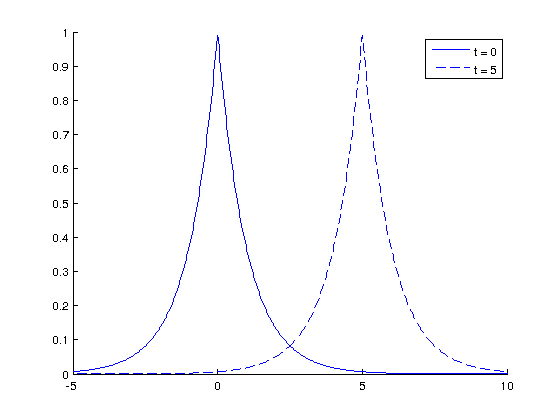
\includegraphics[width=0.8\linewidth]{gfx/peakon}
\end{figure}

\end{frame}


\section{Double peakon}
\begin{frame}

\begin{figure}
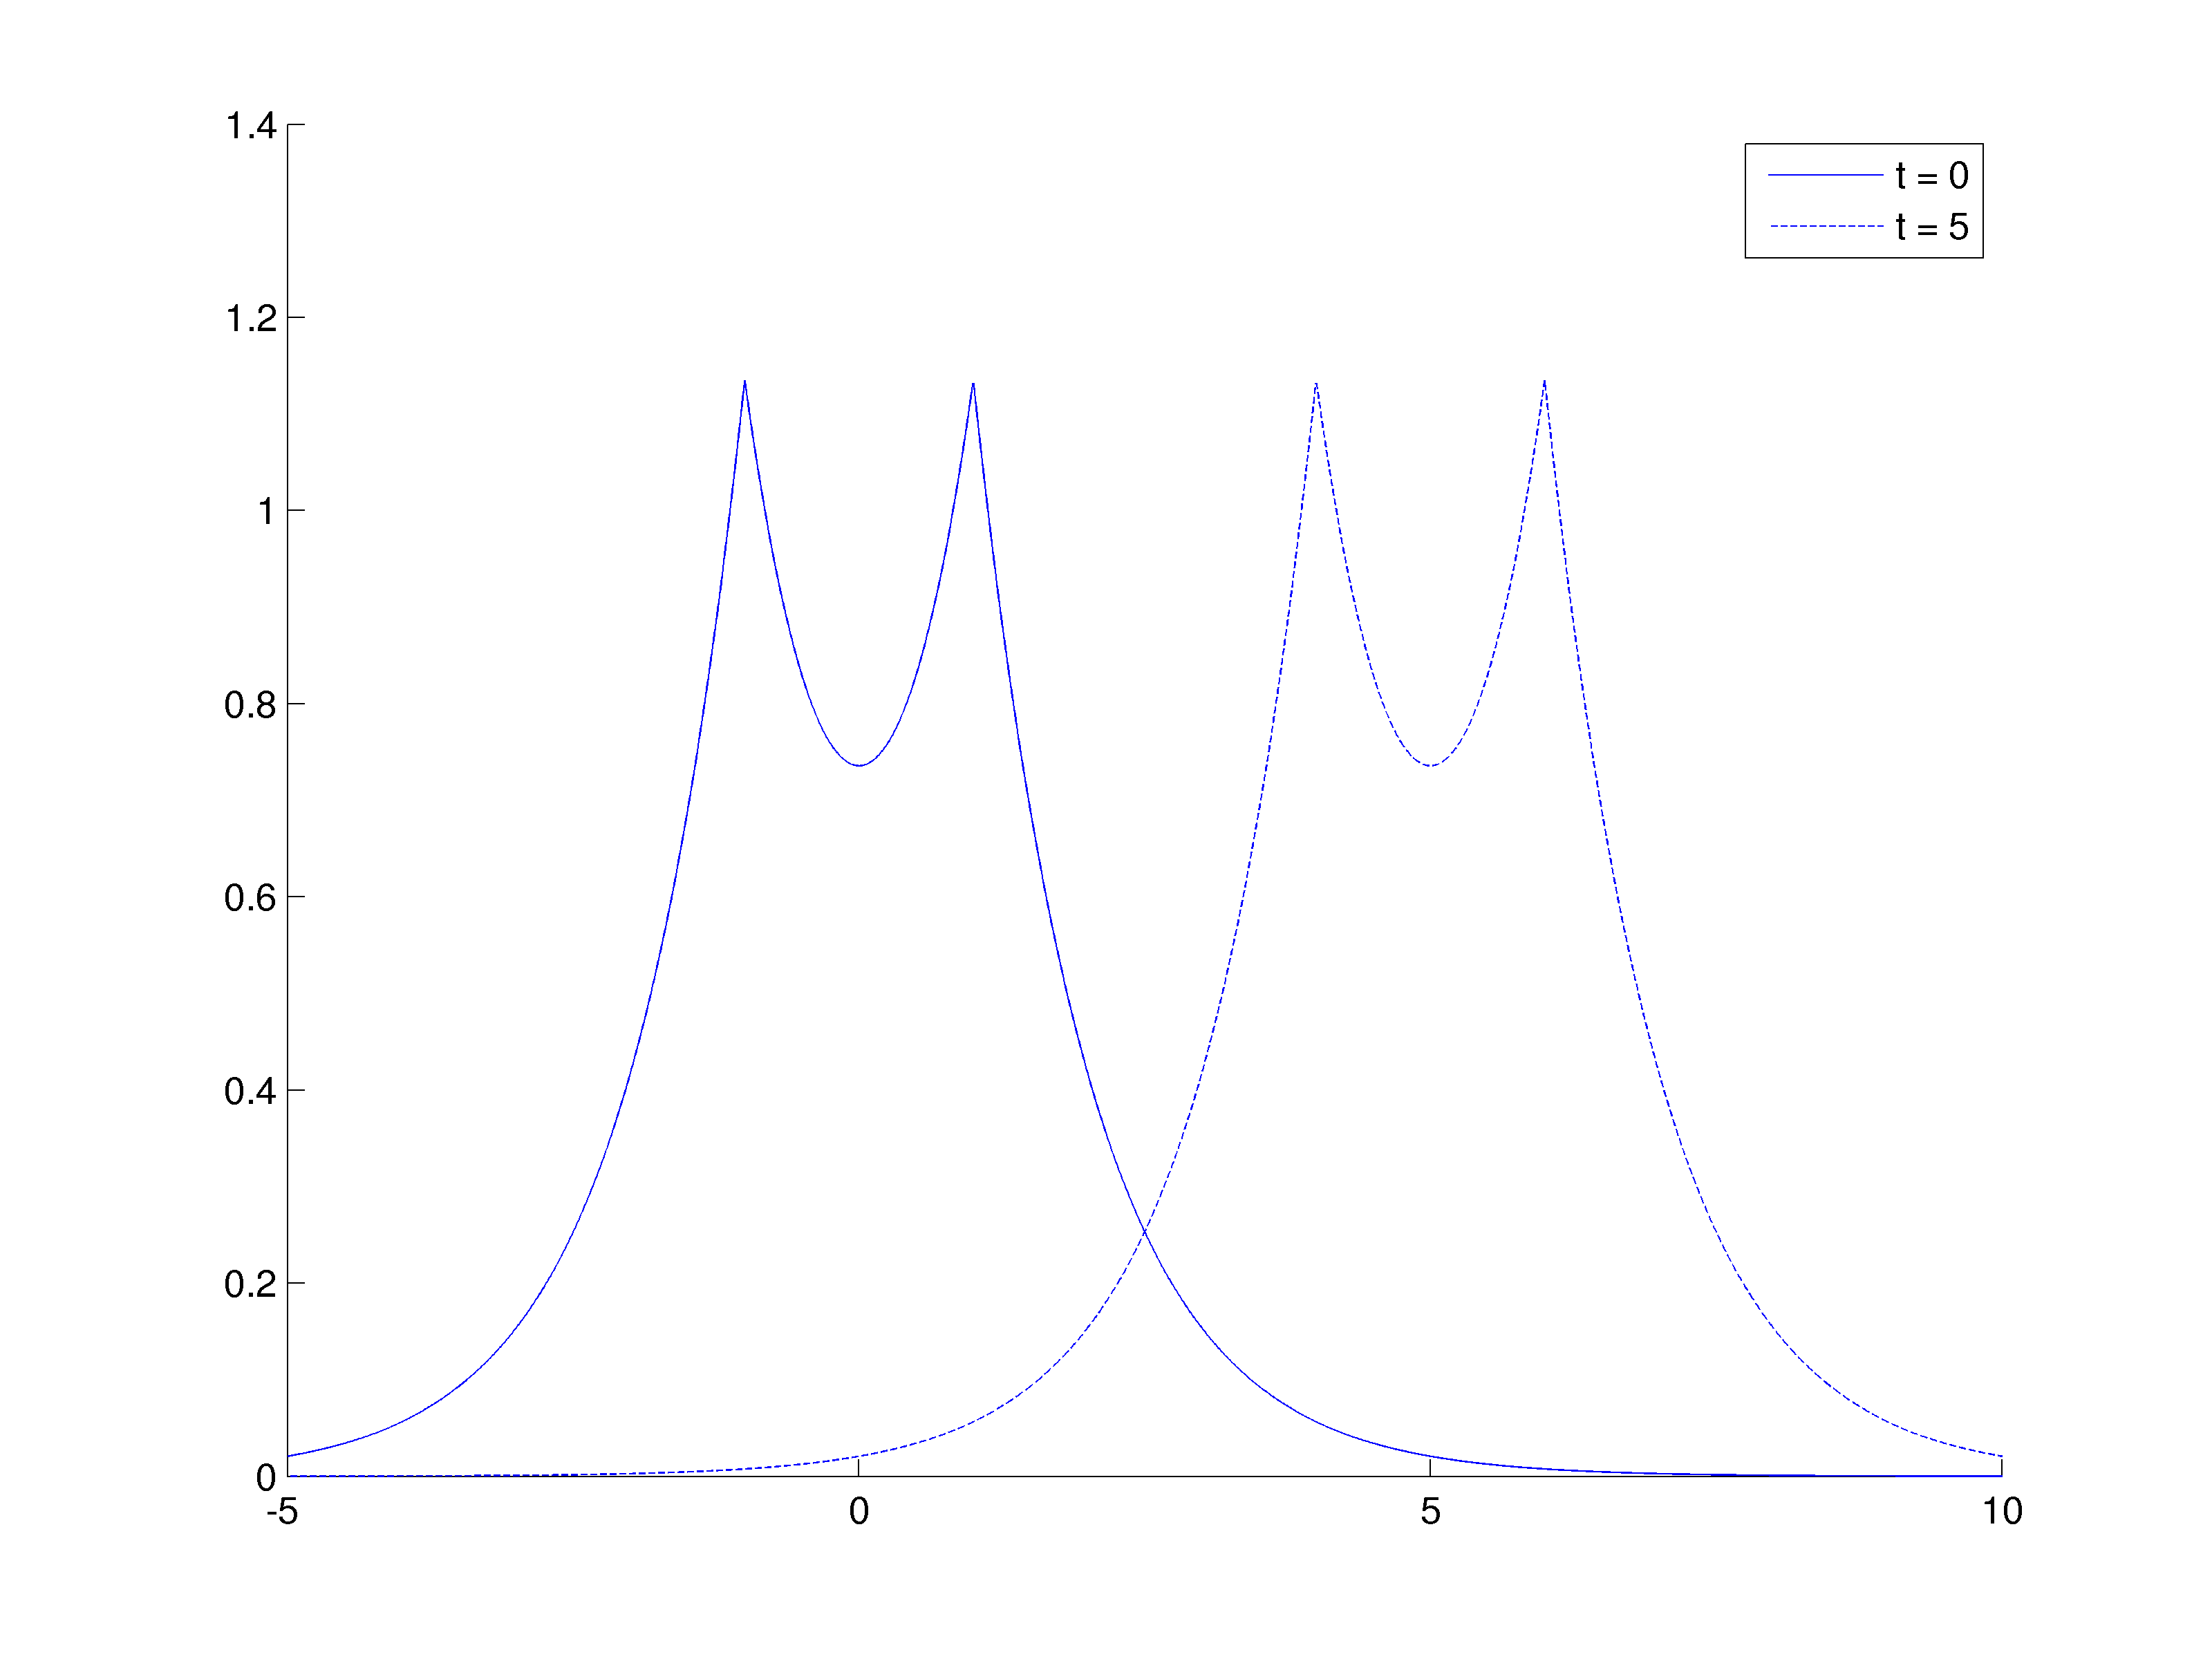
\includegraphics[width=0.8\linewidth]{gfx/doublepeakon}
\end{figure}

\end{frame}


\section{Peakon interaction}
\begin{frame}

\begin{figure}
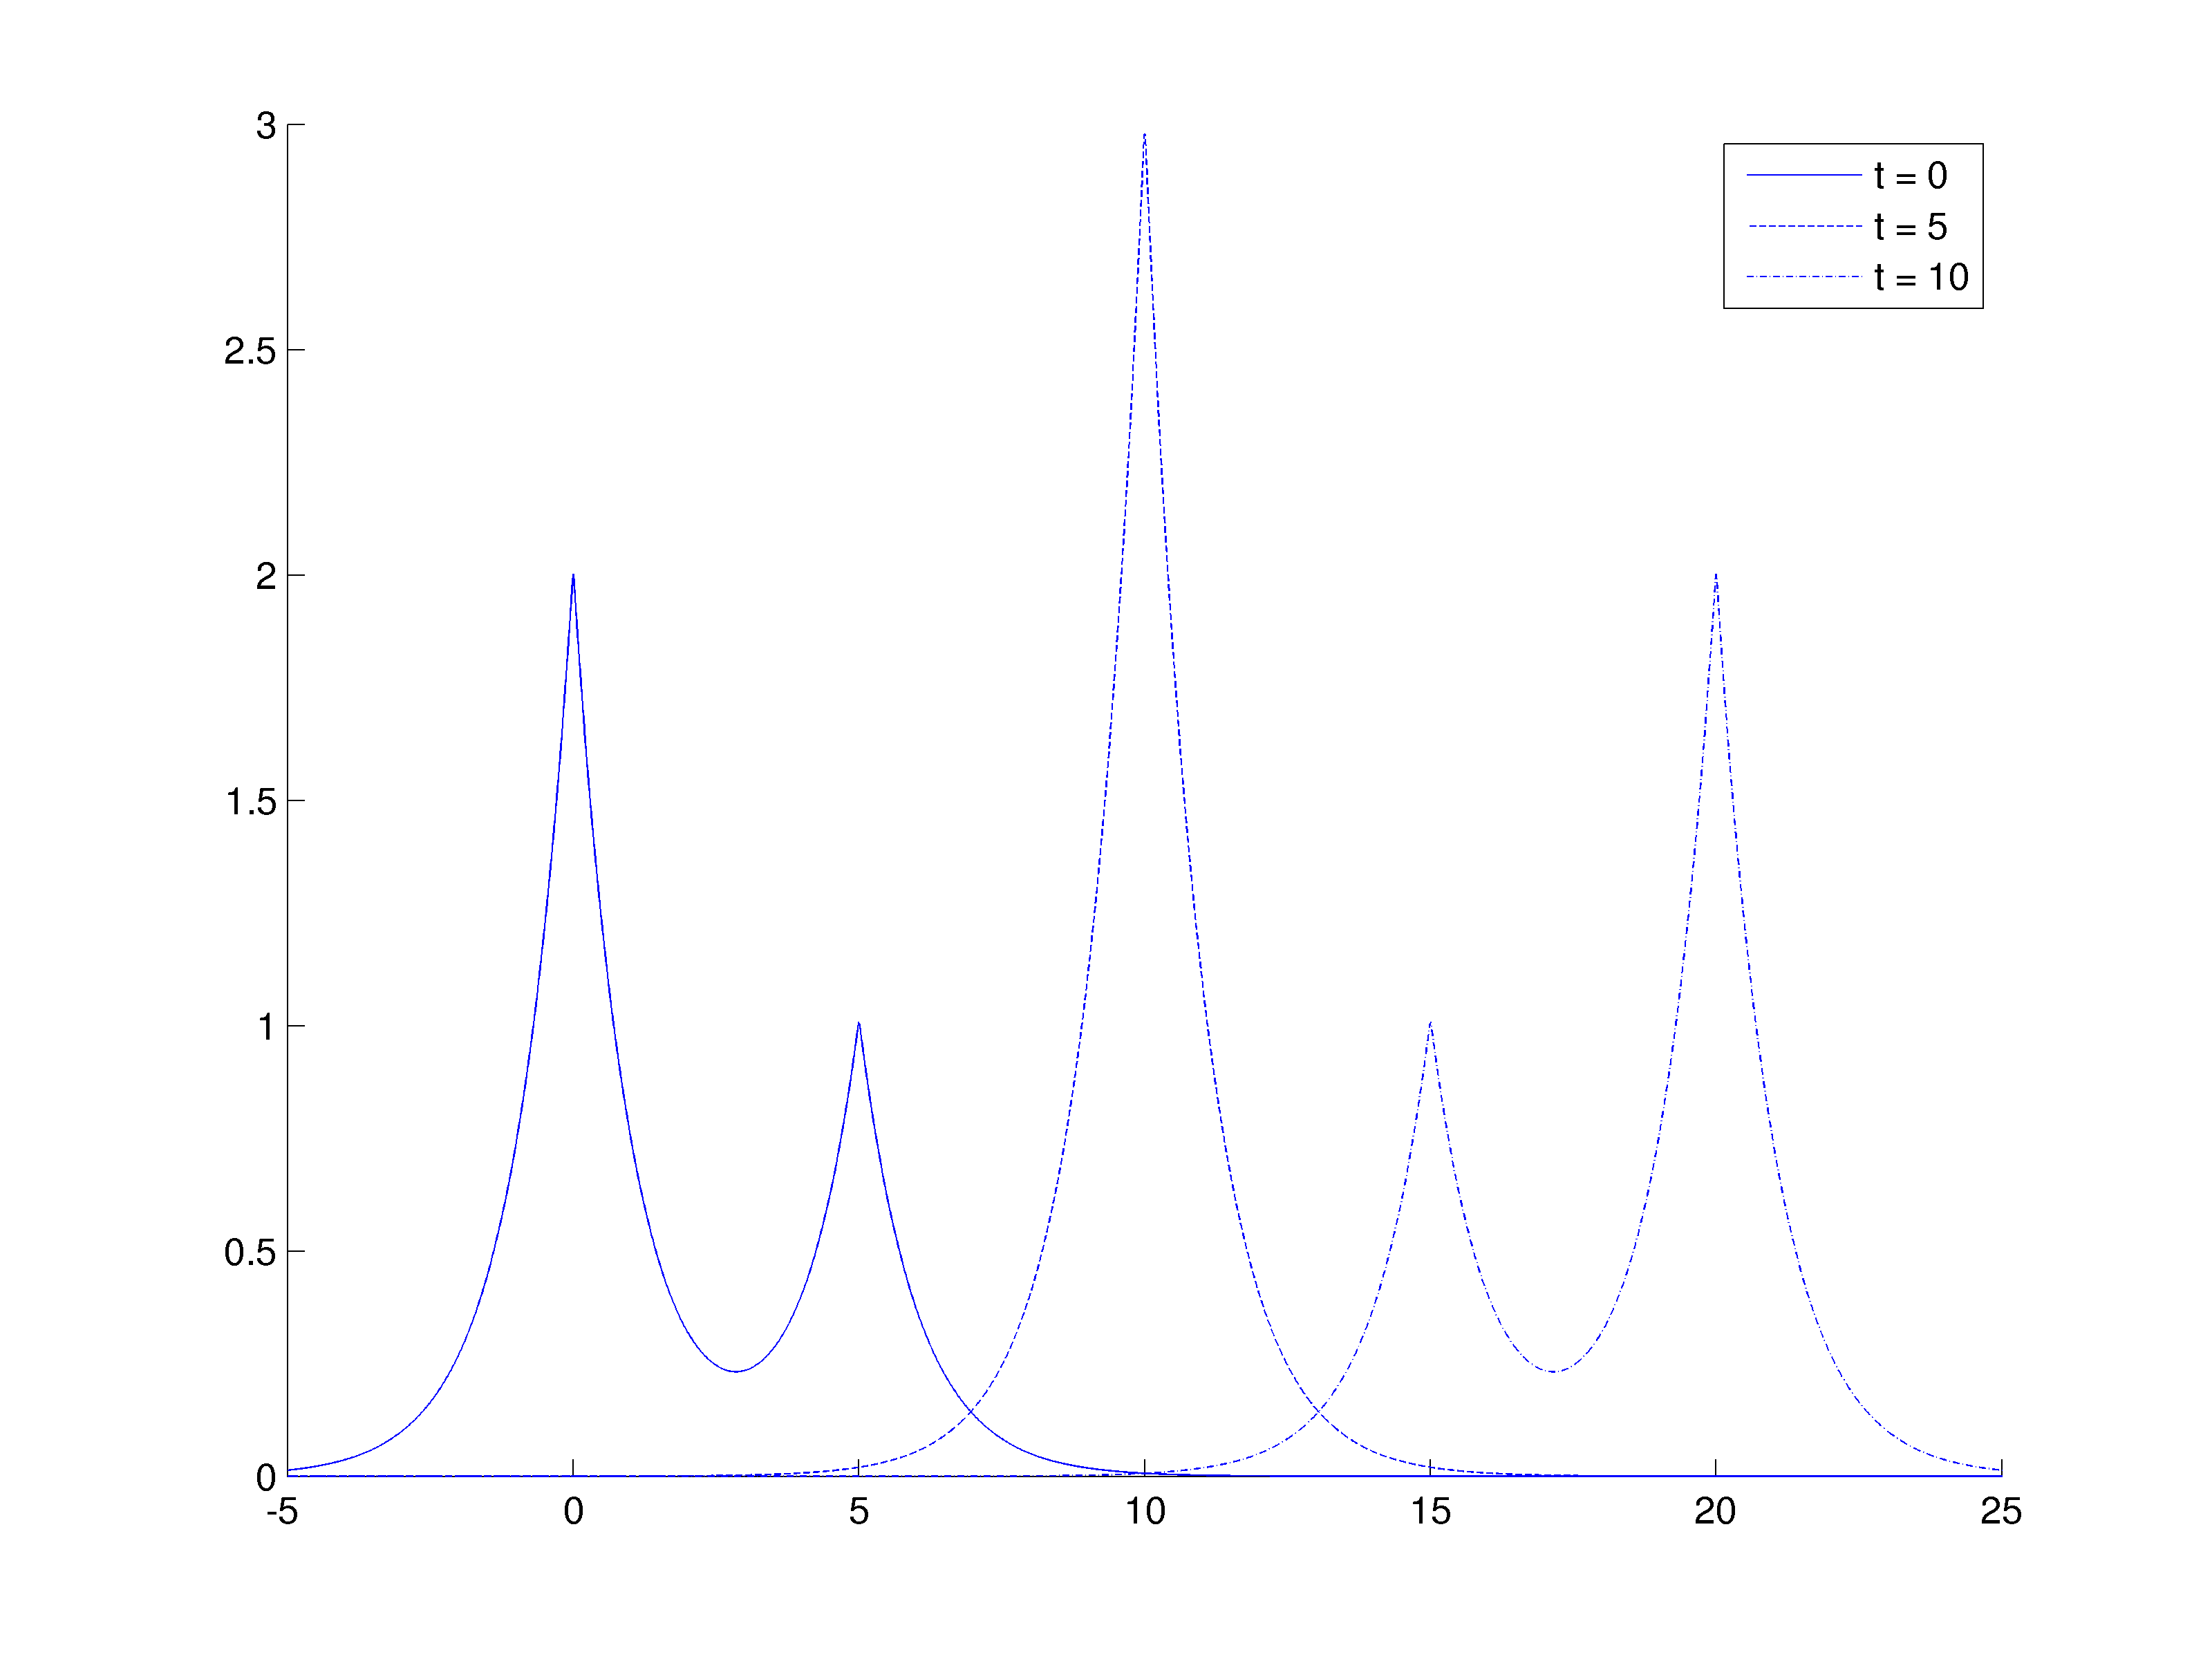
\includegraphics[width=0.8\linewidth]{gfx/peakonovertake}
\end{figure}

\end{frame}


\section{Peakon/antipeakon}
\begin{frame}

\begin{figure}
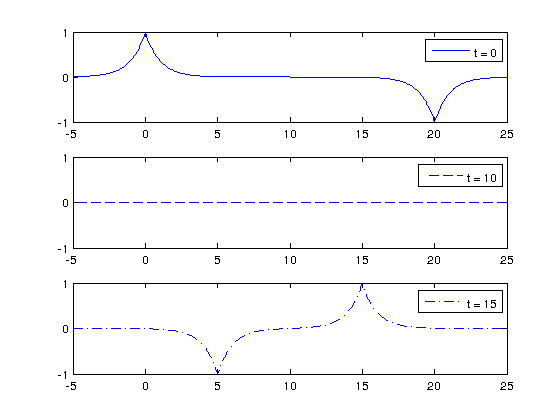
\includegraphics[width=0.8\linewidth]{gfx/peakonantipeakon}
\end{figure}

\end{frame}


\begin{frame}
\frametitle{The finite difference scheme}

\begin{align*}
%m &= Au,\\
m &= u - D_- D_+ u \notag \\
m_t &=- D_- ( m u ) - m D ( u ), 
\end{align*} 

\vspace{3.5cm}

\tiny{H. Holden, X. Raynaud, Convergence of a finite difference scheme for the Camassa-Holm equation}


\end{frame}



\section*{More scheme}
\begin{frame}

\begin{align*}
\bm{M}^{n+1} &= \bm{M}^{n} + k \left[- \bm{B} (\bm{M}^n \circ \bm{U}^n) - \bm{M}^n \circ \bm{D} (\bm{U}^n)\right] \\
\bm{AU}^{n + 1} &= \bm{M}^{n+1}
\end{align*}
\end{frame}



\section*{Extended scheme}
\begin{frame}
\frametitle{Extension of scheme to handle antipeakons}
\begin{align*}
\text{Original} \\
m &= u - D_- D_+ u \notag \\
m_t &=- D_- ( m u ) - m D ( u ), \\ \\
\text{Extended} \\
m &= u - D_{-}D_{+}u, \notag \\ 
m_t &= -D_{-}(m(u \vee 0)) -D_{+}(m(u \wedge 0)) - mD(u), 
\end{align*}

\vspace{1cm}
\tiny{M. L. Dahlby, Geometric integration of nonlinear
wave equations}
\end{frame}


\section*{CFL condition}
\begin{frame}
\frametitle{Necessary condition for stability}
The CFL condition
\begin{align*}
C = \frac{v\Delta t}{\Delta x} \leq C_{\text{max}},
\end{align*}

\end{frame}


\section*{Numerical convergence}
\begin{frame}
\frametitle{Convergence in space}
\begin{figure}
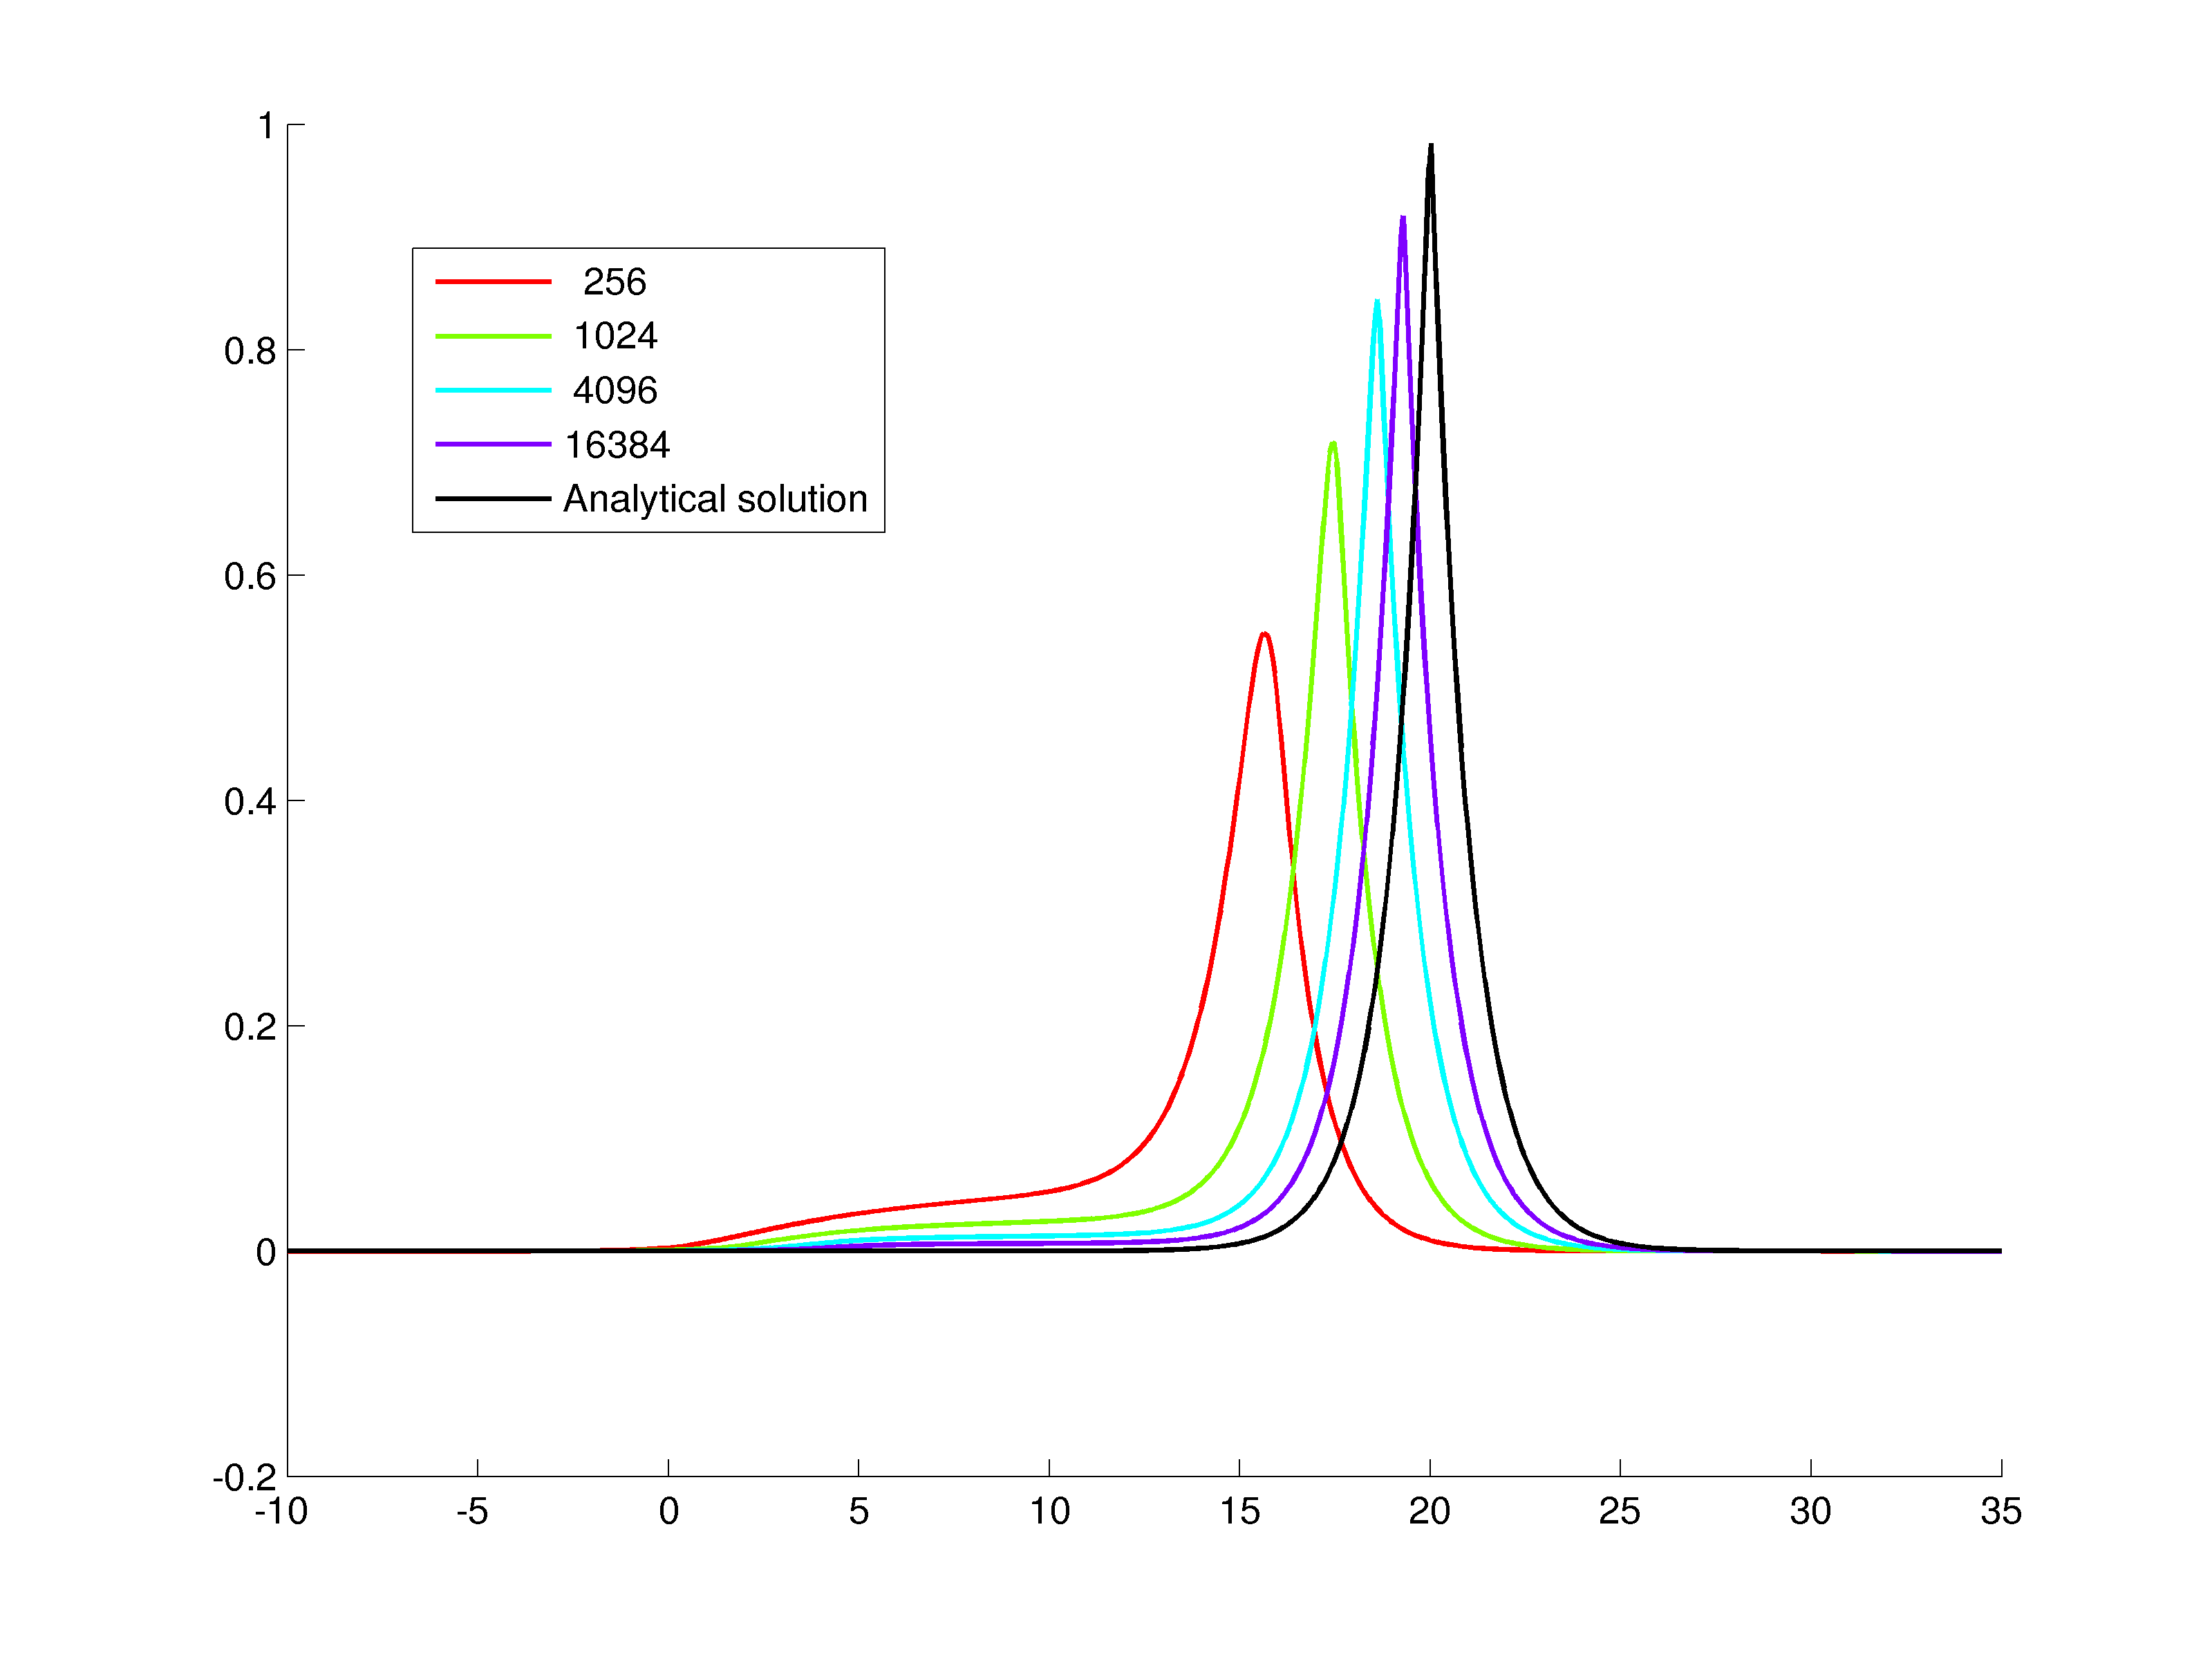
\includegraphics[width=0.8\linewidth]{gfx/attimeT}
\end{figure}
\end{frame}

\section*{Order of convergence}
\begin{frame}
\frametitle{Order of convergence}
\begin{figure}
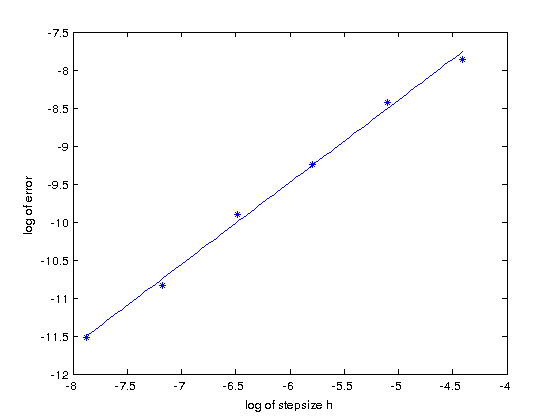
\includegraphics[width=0.8\linewidth]{gfx/loglog}
\end{figure}
\end{frame}

\section*{Analysis}
\begin{frame}
\frametitle{Analysis}
\end{frame}

\section*{Stability}
\begin{frame}
\frametitle{Stability}
\begin{align*}
\bm{m} = \bm{u}-D_-D_+\bm{u} = (\bm{I}-\bm{BF})\bm{u} = \bm{A} \bm{u}
\end{align*} 

\begin{align*}
\bm{m} &= \bm{Au} \\
\bm{m}_t &= -\bm{BMu} - \bm{MCu} = \bm{-Qu},
\end{align*}

\begin{align*}
\bm{m}^{n+1} &= \bm{m} + k\bm{m}_t \\
\bm{m}^{n+1} &= \bm{m} + k\bm{Qu} \\
\bm{u}^{n+1} &= \bm{A^{-1}m^{n+1}} = \left(\bm{I} -\bm{A^{-1}}k\bm{Q}\right)\bm{u} = \bm{Zu}.
\end{align*}
\end{frame}


\begin{frame}
\frametitle{Bullet Points}
\begin{itemize}
\item Lorem ipsum dolor sit amet, consectetur adipiscing elit
\item Aliquam blandit faucibus nisi, sit amet dapibus enim tempus eu
\item Nulla commodo, erat quis gravida posuere, elit lacus lobortis est, quis porttitor odio mauris at libero
\item Nam cursus est eget velit posuere pellentesque
\item Vestibulum faucibus velit a augue condimentum quis convallis nulla gravida
\end{itemize}
\end{frame}

%------------------------------------------------

\begin{frame}
\frametitle{Blocks of Highlighted Text}
\begin{block}{Block 1}
Lorem ipsum dolor sit amet, consectetur adipiscing elit. Integer lectus nisl, ultricies in feugiat rutrum, porttitor sit amet augue. Aliquam ut tortor mauris. Sed volutpat ante purus, quis accumsan dolor.
\end{block}

\begin{block}{Block 2}
Pellentesque sed tellus purus. Class aptent taciti sociosqu ad litora torquent per conubia nostra, per inceptos himenaeos. Vestibulum quis magna at risus dictum tempor eu vitae velit.
\end{block}

\begin{block}{Block 3}
Suspendisse tincidunt sagittis gravida. Curabitur condimentum, enim sed venenatis rutrum, ipsum neque consectetur orci, sed blandit justo nisi ac lacus.
\end{block}
\end{frame}

%------------------------------------------------

\begin{frame}
\frametitle{Multiple Columns}
\begin{columns}[c] % The "c" option specifies centered vertical alignment while the "t" option is used for top vertical alignment

\column{.45\textwidth} % Left column and width
\textbf{Heading}
\begin{enumerate}
\item Statement
\item Explanation
\item Example
\end{enumerate}

\column{.5\textwidth} % Right column and width
Lorem ipsum dolor sit amet, consectetur adipiscing elit. Integer lectus nisl, ultricies in feugiat rutrum, porttitor sit amet augue. Aliquam ut tortor mauris. Sed volutpat ante purus, quis accumsan dolor.

\end{columns}
\end{frame}

%------------------------------------------------
\section{Second Section}
%------------------------------------------------

\begin{frame}
\frametitle{Table}
\begin{table}
\begin{tabular}{l l l}
\toprule
\textbf{Treatments} & \textbf{Response 1} & \textbf{Response 2}\\
\midrule
Treatment 1 & 0.0003262 & 0.562 \\
Treatment 2 & 0.0015681 & 0.910 \\
Treatment 3 & 0.0009271 & 0.296 \\
\bottomrule
\end{tabular}
\caption{Table caption}
\end{table}
\end{frame}

%------------------------------------------------

\begin{frame}
\frametitle{Theorem}
\begin{theorem}[Mass--energy equivalence]
$E = mc^2$
\end{theorem}
\end{frame}

%------------------------------------------------

\begin{frame}[fragile] % Need to use the fragile option when verbatim is used in the slide
\frametitle{Verbatim}
\begin{example}[Theorem Slide Code]
\begin{verbatim}
\begin{frame}
\frametitle{Theorem}
\begin{theorem}[Mass--energy equivalence]
$E = mc^2$
\end{theorem}
\end{frame}\end{verbatim}
\end{example}
\end{frame}

%------------------------------------------------

\begin{frame}
\frametitle{Figure}
Uncomment the code on this slide to include your own image from the same directory as the template .TeX file.
%\begin{figure}
%\includegraphics[width=0.8\linewidth]{test}
%\end{figure}
\end{frame}

%------------------------------------------------

\begin{frame}[fragile] % Need to use the fragile option when verbatim is used in the slide
\frametitle{Citation}
An example of the \verb|\cite| command to cite within the presentation:\\~

This statement requires citation \cite{p1}.
\end{frame}

%------------------------------------------------

\begin{frame}
\frametitle{References}
\footnotesize{
\begin{thebibliography}{99} % Beamer does not support BibTeX so references must be inserted manually as below
\bibitem[Smith, 2012]{p1} John Smith (2012)
\newblock Title of the publication
\newblock \emph{Journal Name} 12(3), 45 -- 678.
\end{thebibliography}
}
\end{frame}

%------------------------------------------------

\begin{frame}
\Huge{\centerline{The End}}
\end{frame}

%----------------------------------------------------------------------------------------

\end{document} 